\section{Gestion de projet}
	\subsection{Courbe en S}
	Tout au long de la session, l’équipe a utilisé Airtable pour faire la division des tâches. Aussi, l’équipe a été capable de suivre facilement la planification initiale grâce à ses suivis hebdomadaires. En effet, chaque jeudi, les tâches du \emph{sprint} finissant étaient discutées et déplacées si nécessaire. La planification du \emph{sprint} à venir était aussi faite, ce qui permettait aux membres de l’équipe de bien prévoir leur temps et leur session de travail. 

	Lors des réunions hebdomadaires, on estimait la durée en heures des tâches planifiées pour le \emph{sprint} à venir en équipe. Les membres étaient assez assidus pour entrer leurs heures travaillées au fur et à mesure. La figure~\ref{fig.courbeS} montre notre courbe en S pour toute la session.
	
	\subsection{Explication de l'allure des courbes}
	Plusieurs tâches ont été réalisées au début du projet jusqu'à la revue~1. Durant cette période, l’équipe a défini le projet et a fait une prévision temporelle du projet pour le restant de la session. Puisque l’équipe a bien suivi cette planification, on voit que l’avancement est linéaire après la revue~1. Il n’y a pas de grande variation des heures travaillées de semaine en semaine.

	L’équipe a aussi été en mesure de ne pas prendre de grand retard durant la session. Cela s’explique à cause que nous avons tenu une gestion hebdomadaire et que s’il y avait un problème avec une tâche, on prenait action immédiatement. 

	Étant donné que l’équipe divisait le projet en petites tâches, l’estimation des heures a été effectuée de manière précise tout au long de la session. Le fait d’utiliser de petites tâches facilitait grandement l’estimation de la durée de la tâche, mais aussi évitait de prendre du retard. En effet, l’avancement des tâches était facile à suivre de semaine en semaine à cause qu’elles prenaient rarement plus de 4~heures à réaliser.
	
	\begin{figure}[H]
		\centering
		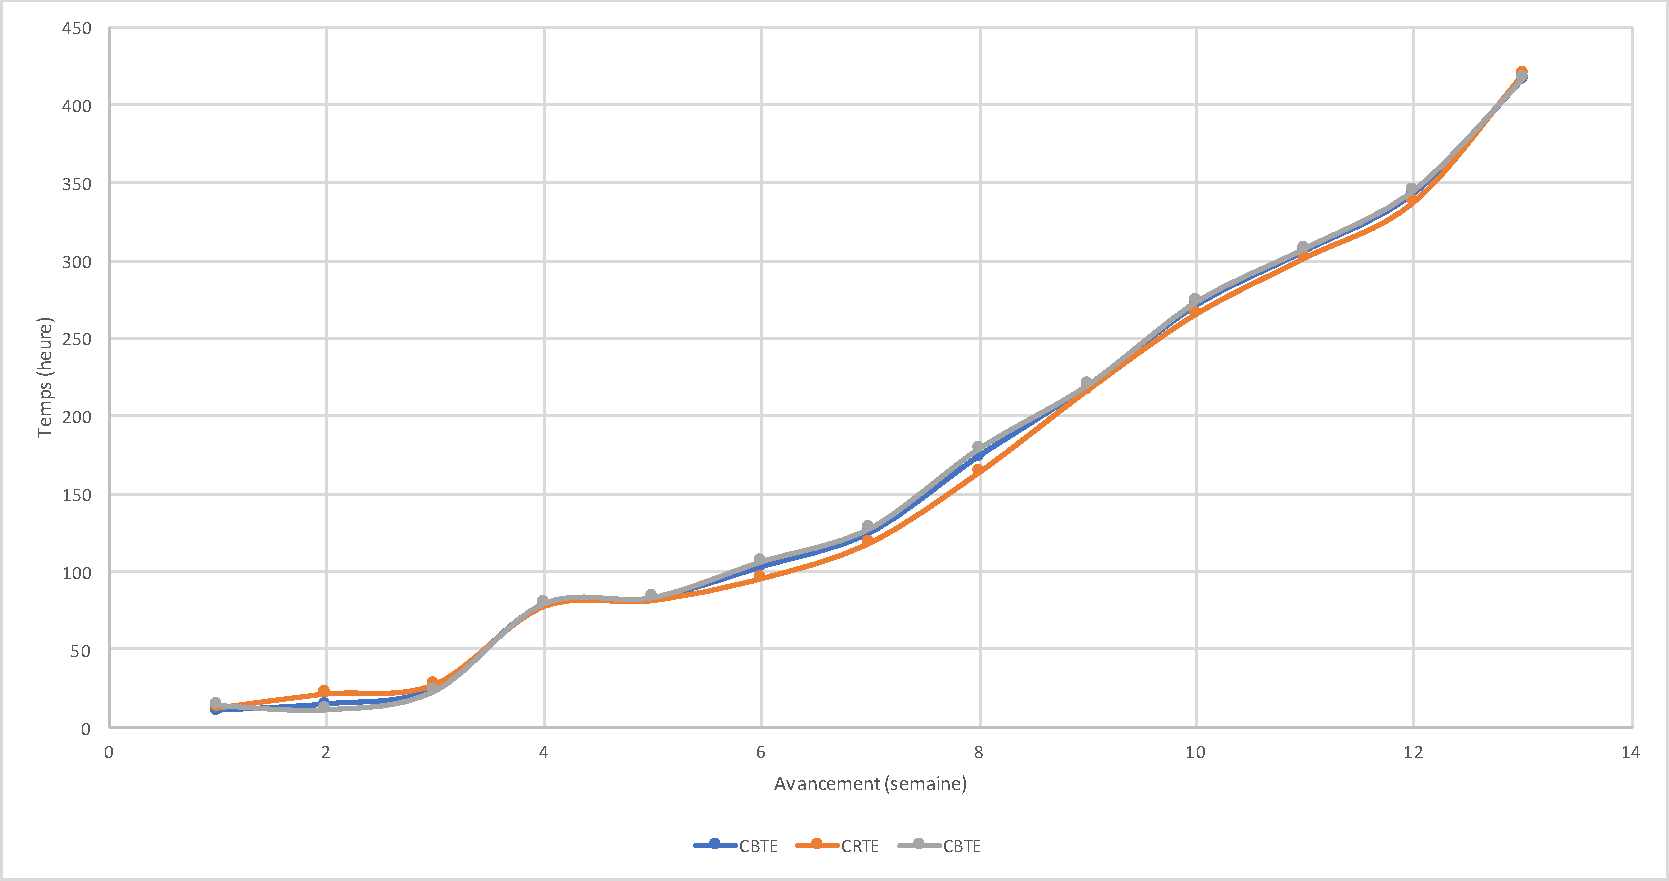
\includegraphics[width=0.9\textwidth]{Pictures/Gestion/courbeS}
		\caption{Courbe en S finale montrant l'évolution temporelle du projet}
		\label{fig.courbeS}
	\end{figure}



%	\begin{landscape}
%	\begin{figure}[p]
%		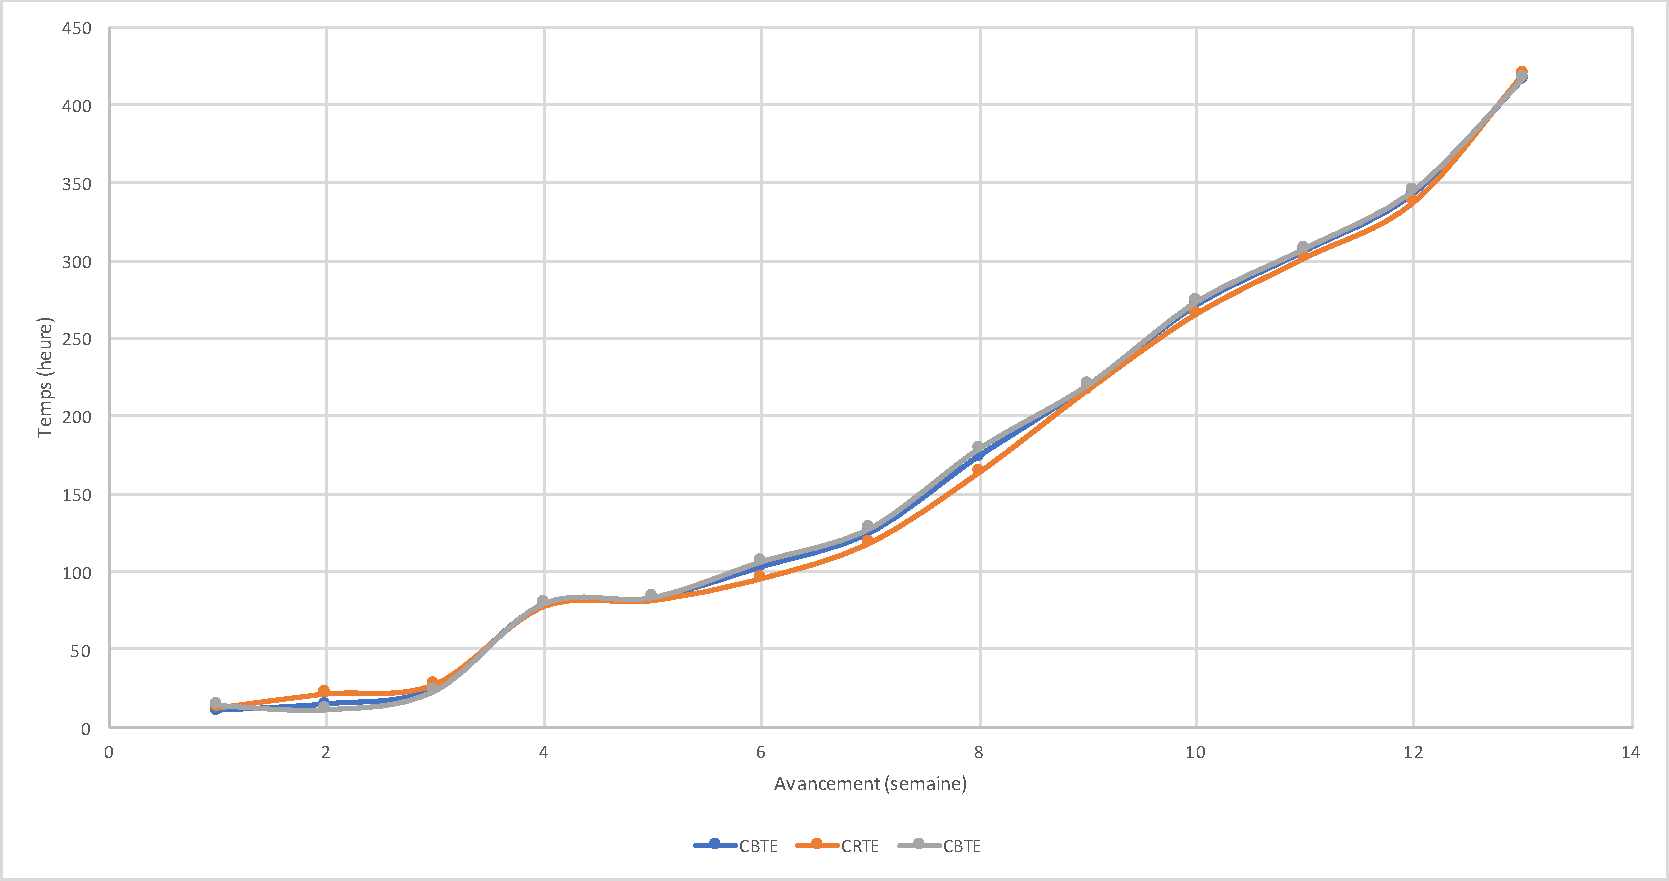
\includegraphics[height=\textheight]{Pictures/Gestion/courbeS}
%		\caption{Courbe en S finale montrant l'évolution temporelle du projet}
%		\label{fig.courbeS}
%	\end{figure}
%	\end{landscape}
